\section{Result I: Counterfactual Actions Require Counterfactual Targets}
\label{sec:actions}

An action-conditioned world model should change its imagined future
when the action sequence changes. Under a teacher-forced JEPA objective
the target encoder observes the trajectory that already contains the
action's effect, which admits an action-invariant solution in which the
predictor matches the target without using the explicit action channel.
We therefore separate two questions. Does the training target make the
action pathway identifiable? Once the pathway is identified, does the
imagined state support an action-dependent downstream readout?

\subsection{Action-Conditioned Predictor}
\label{sec:action-predictor}

The static generator $H$ is replaced by a linear action-conditioned
family~\cite{horowitz2022quantum}
\begin{equation}
H(a) = H_0 + a \cdot H_1,
\qquad U(a) = \exp(-i\, H(a)\, \Delta t),
\label{eq:action-ham}
\end{equation}
with $H_0$ and $H_1$ learnable Hermitian parameters. Discretising
$a \in \{-2, -1, 0, +1, +2\}$ allows the five matrices $U(a)$ to be
pre-computed for the action alphabet and gathered per sample per step.
For an input sequence of actions $(a_t, a_{t+1}, \dots)$ the rollout is
$\hat\rho_{t+k} = U(a_{t+k-1}) \cdots U(a_t) \, \rho_t \, U(a_t)^\dagger
\cdots U(a_{t+k-1})^\dagger$, which uses the same two batched matrix
multiplications per rollout step as the unconditioned predictor plus
an $O(|\mathcal{A}|d^3)$ matrix-exponential precompute for the
discrete action set~\cite{oh2015action,watter2015e2c}.

\subsection{Teacher Forcing Makes Actions Inert}
\label{sec:teacher-forced}

The natural training target for \cref{eq:action-ham} is the
teacher-forced JEPA objective: at each step, match the EMA target
$z_{t+k}^+ = E_\xi(x_{\le t+k})$ produced from the observed trajectory,
which carries the true action history. Under this target,
$\|H_1\| / \|H_0\| \approx 0.03$ at the end of training: the action
channel is driven to near-zero magnitude and $U(a) \approx U(0)$ for
every discrete $a$. Because the observed trajectory already contains
the action's effect and the loss does not distinguish action-sensitive
from action-invariant solutions, the predictor learns to reproduce the
observed trajectory regardless of the action. Teacher forcing alone
leaves the action pathway inert under a JEPA target.

\subsection{Counterfactual Targets Restore Action Binding}
\label{sec:counterfactual}

The fix is to replace the target by a simulator rollout under a
\emph{freshly sampled counterfactual action sequence}
$\tilde a_{t:t+k-1}$~\cite{buesing2018woulda}. Define
\begin{equation}
\tilde\rho_{t+k}^+ \;=\; E_\xi\bigl(x_{\le t} \;\Vert\;
\mathsf{Sim}(s_t, \tilde a_{t:t+k-1})\bigr),
\label{eq:cf-target}
\end{equation}
where $\mathsf{Sim}(s_t, \tilde a_{t:t+k-1})$ is the environment
simulator advanced from the latent simulator state $s_t$ under the
counterfactual actions, and $\Vert$ denotes concatenation of the
observation history. The predictor is then trained to match
$\tilde\rho_{t+k}^+$ when fed $\tilde a_{t:t+k-1}$. Sampling $\tilde a$
independently per batch makes two different action sequences map to
two different targets, so any $H_1$ that is too small incurs loss. The
construction requires simulator-state access during training and is
therefore a controlled test of counterfactual action binding rather
than a recipe for raw video streams without a counterfactual data
source.

After training with the counterfactual target,
$\|H_1\| / \|H_0\| = 1.00 \pm 0.15$ across three seeds: the two terms
in \cref{eq:action-ham} become comparable in magnitude, as expected of
a predictor that uses the action. We refer to this model below as
UWM-JEPA-CF (the suffix CF marks counterfactual-target training) and
to the matched recurrent baseline trained under the same protocol as
LSTM-JEPA-CF.

\subsection{Action Control Battery}
\label{sec:action-controls}

To confirm that the UWM-JEPA-CF predictor actually uses the action channel
(rather than achieving small loss by memorising action-averaged
dynamics), we run action-perturbation controls at test time. Each
condition reports the Hilbert--Schmidt distance from the final
predicted state to the correct counterfactual target; smaller is
better.

\begin{table}[t]
\centering
\footnotesize
\setlength{\tabcolsep}{3pt}
\caption{\textbf{Action perturbation controls on UWM-JEPA-CF.}
Mean $\pm$ std over three seeds. Correct actions give the smallest
distance among test-time perturbations of the same trained model;
wrong, shuffled, and negated actions increase it. The reversed sequence
is a mild perturbation here, so the stronger action-ordering claim rests
on the downstream indicator task. Across the same seeds,
$\|[H_0,H_1]\|/(\|H_0\|\|H_1\|)=0.68\pm0.09$.}
\label{tab:action-controls}
\begin{tabularx}{\columnwidth}{@{}Xr@{}}
\toprule
Test-time action condition & HS distance to target \\
\midrule
Correct actions      & $\mathbf{0.0082 \pm 0.0012}$ \\
Reversed sequence    & $0.0090 \pm 0.0014$ \\
Base dynamics        & $0.0096 \pm 0.0016$ \\
Wrong actions        & $0.0114 \pm 0.0021$ \\
Shuffled actions     & $0.0115 \pm 0.0020$ \\
Negated actions      & $0.0132 \pm 0.0022$ \\
\bottomrule
\end{tabularx}
\end{table}

\subsection{Hidden-Velocity Indicator Task}
\label{sec:indicator}

The counterfactual-target and perturbation results establish that
UWM-JEPA-CF uses the action channel. The indicator task tests whether
this translates into a downstream ability that is absent in the
matched LSTM-JEPA-CF configuration evaluated in the main comparison.

\paragraph{Task}
The indicator is a binary classification: predict
$y = \mathbb{1}[\text{hidden velocity at } t+K > 0]$ with $K = 5$.
The observation at time $t+K$ is masked in the input (observation
stride $3$), so the answer cannot be read off an observed frame. The
model must roll the latent $K$ steps forward \emph{under the action
sequence} and read the sign of velocity from its own imagined state.
The task therefore probes whether the action-conditioned predictor
produces a state from which the hidden continuation is linearly
decodable.

\begin{figure*}[t]
\centering
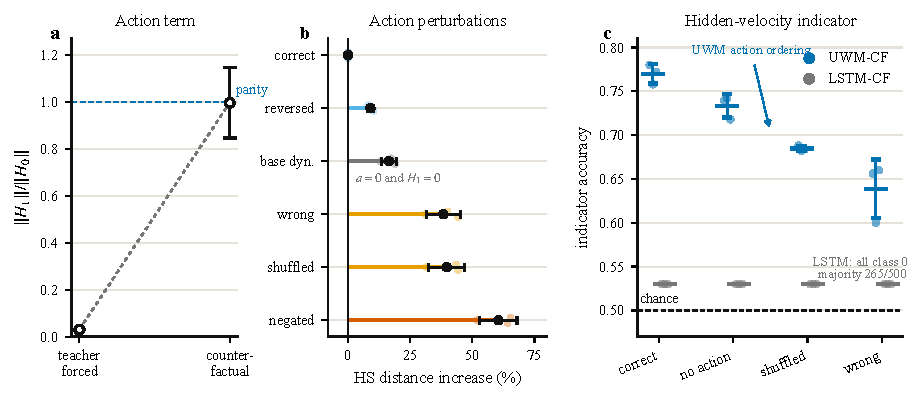
\includegraphics[width=\textwidth]{figures/fig_action_binding_evidence.pdf}
\caption{\textbf{Action-binding evidence.} \textbf{A}: teacher-forced
JEPA makes the action Hamiltonian nearly inert, while counterfactual
targets recover an action term comparable to the base dynamics.
\textbf{B}: action perturbation controls increase Hilbert--Schmidt
distance to the counterfactual target. \textbf{C}: the hidden-velocity
indicator is solved above chance by UWM-JEPA-CF, while the matched
LSTM-JEPA-CF main-comparison configuration collapses to majority-class
predictor.}
\label{fig:action-binding}
\end{figure*}

\begin{table}[t]
\centering
\footnotesize
\setlength{\tabcolsep}{3pt}
\caption{\textbf{Hidden-velocity indicator accuracy.} Values are
mean $\pm$ std over three seeds. UWM-JEPA-CF degrades under action
perturbations; the matched LSTM-JEPA-CF configuration stays at
majority-class accuracy.}
\label{tab:indicator}
\begin{tabularx}{\columnwidth}{@{}lRR@{}}
\toprule
Condition & UWM-JEPA-CF & LSTM-JEPA-CF \\
\midrule
Correct   & $\mathbf{0.770 \pm 0.011}$ & $0.530 \pm 0.000$ \\
No-action & $0.733 \pm 0.013$ & $0.530 \pm 0.000$ \\
Shuffled  & $0.685 \pm 0.003$ & $0.530 \pm 0.000$ \\
Wrong     & $0.639 \pm 0.034$ & $0.530 \pm 0.000$ \\
\bottomrule
\end{tabularx}
\end{table}

\paragraph{Reading}
Three findings emerge (\cref{fig:action-binding}, \cref{tab:indicator}).
First, UWM-JEPA-CF solves the task above chance ($0.770$ with correct
actions) and is action-sensitive: correct exceeds wrong by $13$
percentage points, and the ordering across conditions (correct $>$
no-action $>$ shuffled $>$ wrong) matches physical intuition, since a
wrong action sequence injects the most incorrect velocity signal while
no-action injects none and biases only mildly away from the true
continuation. Second, the parameter-matched LSTM-JEPA-CF, trained on
the same counterfactual JEPA objective with the same action head, is
flat at $0.530$ across all four action conditions: all three
LSTM-JEPA-CF checkpoints predict class $0$ for all $500$ held-out
examples under every action condition, against $265$ class-$0$ and
$235$ class-$1$ ground-truth examples. Third, the scope of the claim
is fixed: under the same JEPA+counterfactual protocol with matched
parameter count, the LSTM variant fails this task while UWM-JEPA-CF
solves it above chance and with the expected action-ordering.

Additional LSTM-CF and supervised recurrent controls are reported in
\cref{sec:baseline-ablations}.
